\documentclass{ximera}

\outcome{Define the average value of a function.}
\outcome{Find the average value of a function.}
\outcome{State the Mean Value Theorem for integrals.}
\outcome{Use the Mean Value Theorem for integrals.}

%\usepackage{todonotes}

\newcommand{\todo}{}

\usepackage{tkz-euclide}
\tikzset{>=stealth} %% cool arrow head
\tikzset{shorten <>/.style={ shorten >=#1, shorten <=#1 } } %% allows shorter vectors

\usepackage{tkz-tab}  %% sign charts
\usetikzlibrary{decorations.pathreplacing} 

\usetikzlibrary{backgrounds} %% for boxes around graphs
\usetikzlibrary{shapes,positioning}  %% Clouds and stars
\usetikzlibrary{matrix} %% for matrix
\usepgfplotslibrary{polar} %% for polar plots
\usetkzobj{all}
\usepackage[makeroom]{cancel} %% for strike outs
%\usepackage{mathtools} %% for pretty underbrace % Breaks Ximera
\usepackage{multicol}

\usepackage{polynom}



\usepackage[many]{tcolorbox}  %% for titled boxes
\newtcolorbox{xbox}[1]{%
    tikznode boxed title,
    enhanced,
    arc=0mm,
    interior style={white},
    attach boxed title to top center= {yshift=-\tcboxedtitleheight/2},
    fonttitle=\bfseries,
    colbacktitle=white,coltitle=black,
    boxed title style={size=normal,colframe=white,boxrule=0pt},
    title={#1}}


\usepackage{array}
\setlength{\extrarowheight}{+.1cm}   
\newdimen\digitwidth
\settowidth\digitwidth{9}
\def\divrule#1#2{
\noalign{\moveright#1\digitwidth
\vbox{\hrule width#2\digitwidth}}}





\newcommand{\RR}{\mathbb R}
\newcommand{\R}{\mathbb R}
\newcommand{\N}{\mathbb N}
\newcommand{\Z}{\mathbb Z}

%\renewcommand{\d}{\,d\!}
\renewcommand{\d}{\mathop{}\!d}
\newcommand{\dd}[2][]{\frac{\d #1}{\d #2}}
\newcommand{\pp}[2][]{\frac{\partial #1}{\partial #2}}
\renewcommand{\l}{\ell}
\newcommand{\ddx}{\frac{d}{\d x}}
\newcommand{\ddt}{\frac{d}{\d t}}

\newcommand{\zeroOverZero}{\ensuremath{\boldsymbol{\tfrac{0}{0}}}}
\newcommand{\inftyOverInfty}{\ensuremath{\boldsymbol{\tfrac{\infty}{\infty}}}}
\newcommand{\zeroOverInfty}{\ensuremath{\boldsymbol{\tfrac{0}{\infty}}}}
\newcommand{\zeroTimesInfty}{\ensuremath{\small\boldsymbol{0\cdot \infty}}}
\newcommand{\inftyMinusInfty}{\ensuremath{\small\boldsymbol{\infty - \infty}}}
\newcommand{\oneToInfty}{\ensuremath{\boldsymbol{1^\infty}}}
\newcommand{\zeroToZero}{\ensuremath{\boldsymbol{0^0}}}
\newcommand{\inftyToZero}{\ensuremath{\boldsymbol{\infty^0}}}



\newcommand{\numOverZero}{\ensuremath{\boldsymbol{\tfrac{\#}{0}}}}
\newcommand{\dfn}{\textbf}
%\newcommand{\unit}{\,\mathrm}
\newcommand{\unit}{\mathop{}\!\mathrm}
\newcommand{\eval}[1]{\bigg[ #1 \bigg]}
\newcommand{\seq}[1]{\left( #1 \right)}
\renewcommand{\epsilon}{\varepsilon}
\renewcommand{\iff}{\Leftrightarrow}

\DeclareMathOperator{\arccot}{arccot}
\DeclareMathOperator{\arcsec}{arcsec}
\DeclareMathOperator{\arccsc}{arccsc}
\DeclareMathOperator{\si}{Si}
\DeclareMathOperator{\proj}{proj}
\DeclareMathOperator{\scal}{scal}


\newcommand{\tightoverset}[2]{% for arrow vec
  \mathop{#2}\limits^{\vbox to -.5ex{\kern-0.75ex\hbox{$#1$}\vss}}}
\newcommand{\arrowvec}[1]{\tightoverset{\scriptstyle\rightharpoonup}{#1}}
\renewcommand{\vec}{\mathbf}
\newcommand{\veci}{\vec{i}}
\newcommand{\vecj}{\vec{j}}
\newcommand{\veck}{\vec{k}}
\newcommand{\vecl}{\boldsymbol{\l}}

\newcommand{\dotp}{\bullet}
\newcommand{\cross}{\boldsymbol\times}
\newcommand{\grad}{\boldsymbol\nabla}
\newcommand{\divergence}{\grad\dotp}
\newcommand{\curl}{\grad\cross}
%\DeclareMathOperator{\divergence}{divergence}
%\DeclareMathOperator{\curl}[1]{\grad\cross #1}


\colorlet{textColor}{black} 
\colorlet{background}{white}
\colorlet{penColor}{blue!50!black} % Color of a curve in a plot
\colorlet{penColor2}{red!50!black}% Color of a curve in a plot
\colorlet{penColor3}{red!50!blue} % Color of a curve in a plot
\colorlet{penColor4}{green!50!black} % Color of a curve in a plot
\colorlet{penColor5}{orange!80!black} % Color of a curve in a plot
\colorlet{fill1}{penColor!20} % Color of fill in a plot
\colorlet{fill2}{penColor2!20} % Color of fill in a plot
\colorlet{fillp}{fill1} % Color of positive area
\colorlet{filln}{penColor2!20} % Color of negative area
\colorlet{fill3}{penColor3!20} % Fill
\colorlet{fill4}{penColor4!20} % Fill
\colorlet{fill5}{penColor5!20} % Fill
\colorlet{gridColor}{gray!50} % Color of grid in a plot

\newcommand{\surfaceColor}{violet}
\newcommand{\surfaceColorTwo}{redyellow}
\newcommand{\sliceColor}{greenyellow}




\pgfmathdeclarefunction{gauss}{2}{% gives gaussian
  \pgfmathparse{1/(#2*sqrt(2*pi))*exp(-((x-#1)^2)/(2*#2^2))}%
}


%%%%%%%%%%%%%
%% Vectors
%%%%%%%%%%%%%

%% Simple horiz vectors
\renewcommand{\vector}[1]{\left\langle #1\right\rangle}


%% %% Complex Horiz Vectors with angle brackets
%% \makeatletter
%% \renewcommand{\vector}[2][ , ]{\left\langle%
%%   \def\nextitem{\def\nextitem{#1}}%
%%   \@for \el:=#2\do{\nextitem\el}\right\rangle%
%% }
%% \makeatother

%% %% Vertical Vectors
%% \def\vector#1{\begin{bmatrix}\vecListA#1,,\end{bmatrix}}
%% \def\vecListA#1,{\if,#1,\else #1\cr \expandafter \vecListA \fi}

%%%%%%%%%%%%%
%% End of vectors
%%%%%%%%%%%%%

%\newcommand{\fullwidth}{}
%\newcommand{\normalwidth}{}



%% makes a snazzy t-chart for evaluating functions
%\newenvironment{tchart}{\rowcolors{2}{}{background!90!textColor}\array}{\endarray}

%%This is to help with formatting on future title pages.
\newenvironment{sectionOutcomes}{}{} 



%% Flowchart stuff
%\tikzstyle{startstop} = [rectangle, rounded corners, minimum width=3cm, minimum height=1cm,text centered, draw=black]
%\tikzstyle{question} = [rectangle, minimum width=3cm, minimum height=1cm, text centered, draw=black]
%\tikzstyle{decision} = [trapezium, trapezium left angle=70, trapezium right angle=110, minimum width=3cm, minimum height=1cm, text centered, draw=black]
%\tikzstyle{question} = [rectangle, rounded corners, minimum width=3cm, minimum height=1cm,text centered, draw=black]
%\tikzstyle{process} = [rectangle, minimum width=3cm, minimum height=1cm, text centered, draw=black]
%\tikzstyle{decision} = [trapezium, trapezium left angle=70, trapezium right angle=110, minimum width=3cm, minimum height=1cm, text centered, draw=black]


\title[Dig-In:]{Applications of integrals}
\begin{document}
\begin{abstract}
We give more contexts to understand integrals.
\end{abstract}
\maketitle



\section{Velocity and displacement, speed and distance}

Some values include ``direction'' that is relative to some fixed point.


  \begin{itemize}
  \item $v(t)$ is the \dfn{velocity} of an object at time $t$. This
    represents the ``change in position'' at time $t$.
  \item $s(t)$ is the \dfn{position} of an object at time $t$. This
    gives location with respect to the origin.     \[
    s(t) = s(a)+\int_a^t v(z) \d z.
    \]
  \item $s(b) -s(a)$ is the \dfn{displacement}, the distance between the
    starting and finishing locations.
  \end{itemize}


On the other hand \textit{speed} and \textit{distance} are values
without ``direction.''


  \begin{itemize}
  \item $|v(t)|$ is the \dfn{speed}.
  \item $\int_a^b |v(t)| \d t$ is the \dfn{distance} traveled.
  \end{itemize}


\begin{question}
  Consider a particle whose velocity at time $t$ is given by $v(t) = \sin(t)$.

\begin{image}
  \begin{tikzpicture}[
      declare function = {f(\x) = sin(deg(\x));}]
    \begin{axis}[  
        domain=-.2:7, xmin =-.2,xmax=7,ymax=1.2,ymin=-1.2,
        width=6in,
        height=3in,xtick={3.141,6.282},
        xticklabels={$\pi$, $2\pi$},
        ytick style={draw=none},
        yticklabels={},
        axis lines=center, xlabel=$x$, ylabel=$y$,
        every axis y label/.style={at=(current axis.above origin),anchor=south},
        every axis x label/.style={at=(current axis.right of origin),anchor=west},
        axis on top,
      ]
               \addplot [ultra thick,penColor, smooth] {f(x)};
    \end{axis}
  \end{tikzpicture}
\end{image}
What is the displacement of the particle from $t=0$ to $t=\pi$? That
is, compute:
\[
\int_0^\pi \sin(t) \d t \begin{prompt}= \answer[given]{2}\end{prompt}
\]
What is the displacement of the particle from $t=0$ to $t=2\pi$? That is, compute:
\[
\int_0^{2\pi} \sin(t) \d t \begin{prompt}= \answer[given]{0}\end{prompt}
\]
What is the distance traveled by the particle from $t=0$ to $t=\pi$?
That is, compute:
\[
\int_0^\pi  \left| \sin(t) \right|  \d t \begin{prompt}= \answer[given]{2}\end{prompt}
\]
What is the distance traveled by the particle from $t=0$ to $t=2\pi$?
That is, compute:
\[
\int_0^{2\pi} \left| \sin(t) \right| \d t \begin{prompt}=\answer[given]{4}\end{prompt}
\]
\end{question}

\section{ Change in the  amount }

We can apply the Fundamental Theorems of Calculus to a variety of problems where both accumulation and rate of change play important roles.
For example, we can consider a tank that is being filled with fuel at some rate. Given the rate, we can ask what is the amount of fuel in the tank  at a  certain time.
Or, a tank that is being emptied at a given rate, or  a culture of bacteria growing in a Petri dish, or a  population of a city, etc.
This brings us to our next theorem.


\begin{theorem}\hfill

Let  $A(t)$ denote the amount of some substance/population at the time $t$.

 Assume that the function $A$ is continuous, differentiable and its derivative, $A'$, continuous on some time interval $[a,b]$.
 
 
Then, the \textbf{change} in the amount $A$ over the time interval $[a,b]$ is given by
\[
A(b)-A(a)=\int_a^bA'(t)dt.
\]
\end{theorem}
\begin {explanation}
The equation follows directly from the Second Theorem of Calculus. 
The left hand side obviously gives the change in the amount $A$ over the time interval $[a,b]$, which is the difference between the amount at the end of the time interval and the amount at the beginning of the time interval. 

The right hand side of the equation gives the ``accumulation of a rate".
You can think of this definite integral as the limit of Riemann sums, where each Riemann sum is the``sum of  the changes of the amount over small intervals of time".
\end {explanation}

\begin{example}
An experiment is conducted in which a culture of bacteria is grown in a Petri dish. The initial population was  estimated at 1200 cells. 
The  growth rate of the population is estimated at  $P'(t)=100e^{-0.2 t}$ cells/day.
\begin{enumerate}
\item By how much has the population grown during the first three days of the experiment?
\begin{explanation}
The growth of population during the first three days of the experiment is given by:
\begin{align*}
  P(3)-P(0) &=\int_0^3 P'(t)\d t\\
  &=\int_0^3 100 e^{-0.2 t}\d t\\
  &=\eval{\frac{100}{-0.2}e^{-0.2 t}}_0^3\approx 226
\end{align*}
During the first three  days, the population  grew  approximately by 226 cells. 
\end{explanation}

\item 
Compute the right Riemann sum of the function $P'$ and the interval $[0,3]$ with $n=3$.
What does this Riemann sum approximate?  Is this approximation an underestimate or an overestimate and why?


\begin{explanation}
This Riemann sum approximates the change in population during the first three days of the experiment.
We expect it to be an underestimate, because the function $P'$ is decreasing and this is a right Riemann sum.

Since $n=3$,  $\Delta t=1$.
\begin{align*}
  P(3)-P(0) &\approx\sum_{k=1}^3P'(k)\\
  &=P'(1)+P'(2)+P'(3)\\
  &=100e^{-0.2 }+100e^{-0.4}+100e^{-0.6}\\
  &\approx 204
\end{align*}
\end{explanation}
\item Find the population at any time $t\ge0$.
\begin{explanation}
\begin{align*}
  P(t)-P(0)&=\int_0^t P'(z)\d z\\
  &=\int_0^t 100 e^{-0.2 z}\d z\\
  &=\eval{\frac{100}{-0.2}e^{-0.2 z}}_0^t\\
  &=500\left(1-e^{-0.2 t}\right)
\end{align*}
Therefore, for $t\ge0$,
\[
P(t)=P(0)+500\left(1-e^{-0.2 t}\right)=1700 -500e^{-0.2 t}
\]
\end{explanation}
\end{enumerate}
\end{example}

\section{Average value}

Conceptualizing definite integrals as ``signed area'' works great as
long as one can actually visualize the ``area.'' In some cases, a
better metaphor for integrals comes from the idea of \textit{average
  value}.  Looking back to your days as an even younger mathematician,
you may recall the idea of an \textit{average}:
\[
\frac{f_1+f_2+\dots+f_n}{n} = \frac{1}{n}\sum_{k=1}^n f_k
\]
If we want to know $\overline{f}$, the average value of a function on the interval $[a,b]$, a naive approach
might be to introduce $n+1$ equally spaced
grid points on the interval $[a,b]$
\[
a=x_0 < x_1 < \dots < x_{n}=b
\]
and choose a sample point $x_k^*$ in  each interval $[x_k,x_{k+1}]$, $k=1,\dots,n$. 

We will approximate the average value of $f$ on the interval $[a,b]$ with the average of $f(x_1^*)$,
$f(x_2^*)$, \dots, and  $f(x_n^*)$:
\[
\overline{f}\approx\frac{f(x_1^*) + f(x_2^*) + \dots + f(x_n^*)}{n} = \frac1n\sum_{k=1}^n f(x_k^*).
\]
Multiply this last expression by $1 = \frac{(b-a)}{(b-a)}$:
\begin{align*}
  \frac1n \sum_{k=1}^n f(x_k^*)\frac{(b-a)}{(b-a)} &= \sum_{k=1}^n f(x_k^*)\frac1n \frac{(b-a)}{(b-a)} \\
  &= \frac{1}{b-a} \sum_{k=1}^n f(x_k^*)\frac{b-a}n  \\
  &=\frac{1}{b-a} \sum_{k=1}^n f(x_k^*)\Delta x
\end{align*}
where $\Delta x = (b-a)/n$.  Ah! On the right we have a Riemann Sum!

What will happen  as $n\to\infty$?

We take the limit as $n\to\infty$:
\[
\overline{f}=\lim_{n\to\infty} \frac{1}{b-a} \sum_{k=1}^n f(x_k^*)\Delta x = \frac{1}{b-a} \int_a^b f(x)\d x.
\]
This leads us to our next definition:

\begin{definition}
  Let $f$ be continuous on $[a,b]$. The \dfn{average value} of $f$ on
  $[a,b]$ is given by
  \[
\overline{f}=  \frac{1}{b-a}\int_a^b f(x)\d x.
  \]
\end{definition}
Multiplying this equation by $(b-a)$, we obtain that 
 \[
\overline{f}(b-a)= \int_a^b f(x)\d x.
  \]
If $f$ is positive,  the average value of a function gives the  height of a single rectangle whose  area is equal to
\[
\int_a^b f(x) \d x.
\]
\begin{image}
  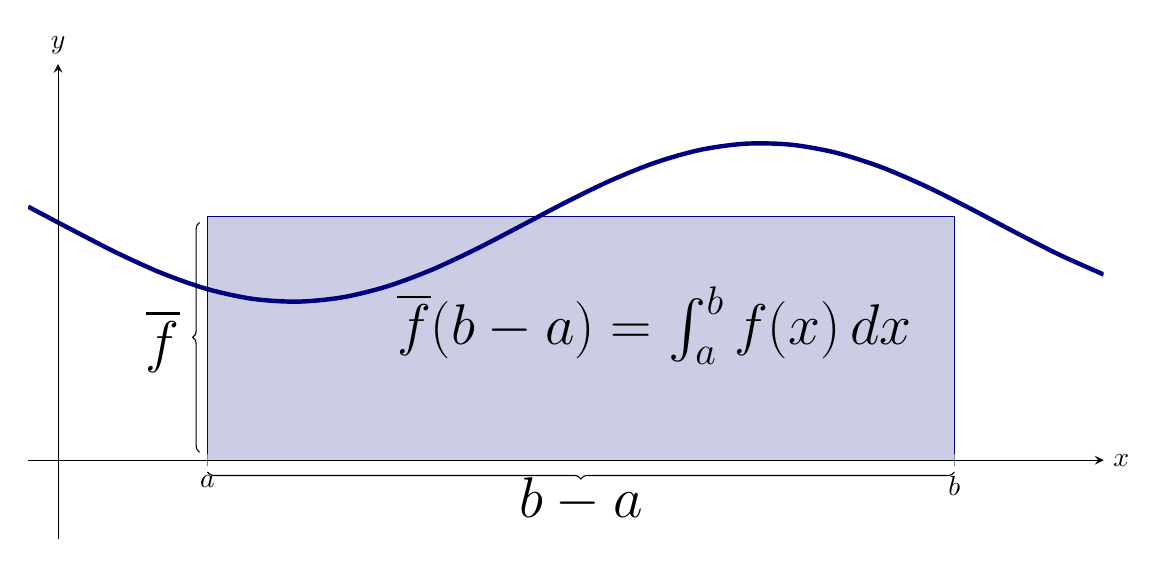
\begin{tikzpicture}[
      declare function = {f(\x) = -sin(deg(\x)) + 3;}]
    \begin{axis}[  
        domain=-.2:7, xmin =-.2,xmax=7,ymax=5,ymin=-1,
        width=6in,
        height=3in,xtick={1,6},
        xticklabels={$a$,$b$},
        ytick style={draw=none},
        yticklabels={},
        axis lines=center, xlabel=$x$, ylabel=$y$,
        every axis y label/.style={at=(current axis.above origin),anchor=south},
        every axis x label/.style={at=(current axis.right of origin),anchor=west},
        axis on top,
      ]
      \foreach \rectnumber in {1}
               {
                 \addplot [draw=penColor,fill=fillp] plot coordinates
                          {({1+(\rectnumber - 1) * 5},{3.08})
                            ({1+(\rectnumber) * 5},{3.08})} \closedcycle;
               };
               \addplot [ultra thick,penColor, smooth] {f(x)};
                \addplot[decoration={brace,raise=.1cm},decorate,thin] plot coordinates
                       {(1,.1) (1,3)};
               \addplot[decoration={brace,mirror,raise=.1cm},decorate,thin] plot coordinates
                       {(1,-0.05) (6,-0.05)};
                         \node[black] at (axis cs:3.99,1.7) {\huge$\overline{f}(b-a)=\int_a^bf(x)\d x$};
               \node[black] at (axis cs:3.5,-0.5) {\huge$b-a$};
                \node[black] at (axis cs:0.7,1.5) {\huge$\overline{f}$};
    \end{axis}
  \end{tikzpicture}
\end{image}

An application of this definition is given in the next example.


\begin{example}
An object moves back and forth along a straight line with a velocity
given by $v(t) = (t-1)^2$ on $[0,3]$, where $t$ is measured in seconds
and $v(t)$ in ft/s.

What is the average velocity of the object?
\begin{explanation}
By our definition, the average velocity is:
\begin{align*}
\overline{v}&=\frac{1}{3-0}\int_0^3v(t)\d t\\
&=\frac{1}{3}\int_0^3 (t-1)^2\d t \\
&=\frac13 \int_0^3 (t^2-2t+1)\d t&=\\
&= \frac13\eval{\frac{t^3}{3}-t^2+t}_0^3\\
&= 1\text{ ft/s}.
\end{align*}
\end{explanation}
\end{example}
\begin{question}
Choose \textbf{all} the correct expressions for $\overline{v}$, the average velocity of an object moving along a straight line over the time interval $[a,b]$.

(Reminder: $s$ is the position function, and $a$ the acceleration). 
\begin{selectAll}
\choice{$\overline{v}=\frac{1}{b-a}\int_a^b s(t)\d t$}

\choice[correct]{$\overline{v}=\frac{1}{b-a}\int_a^b v(t)\d t$}

\choice{$\overline{v}=\frac{1}{b-a}\int_a^b a(t)\d t$}

\choice{$\overline{v}=\frac{a(b)-a(a)}{b-a}$}


\choice{$\overline{v}=\frac{v(b)-v(a)}{b-a}$}
\choice[correct]{$\overline{v}=\frac{s(b)-s(a)}{b-a}$}

\end{selectAll}
\begin{feedback}
We know from before that
\[
\overline{v}=\frac{s(b)-s(a)}{b-a}.
\]
We also know that the position function is given by
\[
s(t)=s(a)+\int_a^tv(z)\d z.
\]
Therefore,
\[
\overline{v}=\frac{s(b)-s(a)}{b-a}=\frac{s(a)+\int_a^bv(t)\d t-s(a)}{b-a}=\frac{1}{b-a}\int_a^bv(t)\d t.
\]
Therefore, we can compute the average velocity using either the position function or the velocity function.
\end{feedback}
\end{question}


When we take the average of a finite set of values, it does not matter
how we order those values.  When we are taking the average value of a
function, however, we need to be more careful.

For instance, there are at least two different ways to make sense of a
vague phrase like ``The average height of a point on the unit semi
circle''
\begin{image}
  \begin{tikzpicture}[
      declare function = {f(\x) = sin(deg(\x));}]
    \begin{axis}[  
        domain=-3:3, xmin =-1.2,xmax=1.2,ymax=1.2,ymin=-.2,
        width=6in,
        height=4in,xtick={-1,1},
        xticklabels={$-1$, $1$},
        ytick style={draw=none},
        yticklabels={},
        axis lines=center, xlabel=$x$, ylabel=$y$,
        every axis y label/.style={at=(current axis.above origin),anchor=south},
        every axis x label/.style={at=(current axis.right of origin),anchor=west},
        axis on top,
      ]
              \addplot [penColor, ultra thick, smooth, domain=(0:180)] ({cos(x)},{sin(x)});
    \end{axis}
  \end{tikzpicture}
\end{image}
One way we can make sense of ``The average height of a point on the
unit semi circle'' is to compute the average value of the function
\[
f(x) =\sqrt{1-x^2}
\]
on the interval $[-1,1]$.

\begin{example}
  Compute the average value of the function
  \[
  f(x) =\sqrt{1-x^2}
  \]
  on the interval $[-1,1]$.
  \begin{explanation}
    By definition, we wish to compute
    \[
    \frac{1}{2}\int_{-1}^1 \sqrt{1-x^2} \d x.
    \]
    Computing this integral geometrically, we find the average value
    to be $\answer[given]{\frac{\pi}{4}}$.
  \end{explanation}
\end{example}
Another way we can make sense of ``The average height of a point on the
unit semi circle'' is the average value of the function
\[
g(\theta) =\sin(\theta)
\]
on $[0,\pi]$, since $\sin(\theta)$ is the height of the point on the
unit circle at the angle $\theta$.
\begin{example}
  Compute the average value of the function
  \[
  g(\theta) =\sin(\theta)
  \]
  on the interval $[0,\pi]$.
  \begin{explanation}
    By definition, we wish to compute
    \[
    \frac{1}{\pi} \int_0^\pi\sin(\theta) \d \theta.
    \]
    Computing this integral geometrically, we find the average value
    to be $\answer[given]{\frac{2}{\pi}}$.
  \end{explanation}
\end{example}

See if you can understand intuitively why the average using $f$ should
be larger than the average using $g$.  %% It is amusing to note that
%% since
%% \[
%% g(x) < f(x)
%% \]this
%% shows that $\pi^2>8$.



\section{Mean value theorem for integrals}

Just as we have a Mean Value Theorem for Derivatives, we also have a
Mean Value Theorem for Integrals.


\begin{theorem}[The Mean Value Theorem for integrals]\index{Mean Value Theorem for integrals}
Let $f$ be continuous on $[a,b]$. There exists a value $c$ in $(a,b)$
such that
\[
\int_a^bf(x)\d x = f(c)(b-a).
\]
\end{theorem}

This is an \emph{existential} statement. The Mean Value Theorem for
Integrals tells us:
\begin{quote}
\textbf{The average value of a continuous function is in the range of
  the function.}
\end{quote}
\begin{proof}
Define an accumulation (area) function, $F$,
\[
F(x)= \int_a^x f(t)\d t 
\]
Since $F$ is continuous on the interval $[a,b]$ and differentiable on the interval $(a,b)$, we can apply the Mean Value Theorem to the function $F$ on the interval $[a,b]$.
Therefore, there exist a number $c$ in $(a,b)$ such that
\[
F'(c)=\frac{F(b)-F(a)}{b-a}
\]
But we know that $F'(c)=f(c)$, and that $F(b)-F(a)=\int_a^bf(t)\d t =\int_a^bf(x)\d x $.
Therefore,
\[
f(c)=\frac{1}{b-a}\int_a^bf(x)\d x
\]
\end{proof}
We demonstrate the principles involved in this version of the Mean
Value Theorem in the following example.

\begin{example}%%%BADBAD we state that this is an existential thm, then we ask for the value!
  Let $f(x)=\sin{x}$. Consider $\int_0^\pi \sin x \d x$. Find a value $c$ guaranteed by the Mean Value Theorem.
  \begin{explanation}
    We first need to evaluate $\int_0^\pi \sin x\d x$.
    \[
    \int_0^\pi\sin x\d x =\eval{-\cos x}_0^\pi = 2.
    \]
    Thus we seek a value $c$ in $[0,\pi]$ such that $\pi\sin c =2$. 
    \[
    \pi\sin c = 2\ \ \Rightarrow\ \ \sin c = 2/\pi\ \ \Rightarrow\ \ c_1 = \arcsin(2/\pi) \approx 0.69.
    \]
    There is another  such point: $c_2=\pi-0.69$.
   Indeed,
    \[
    f( \pi-0.69)=\sin{(\pi-0.69)}=\sin{(0.69)}=\frac{2}{\pi}=\overline{f}.
    \]
A graph of $\sin x$, along with a rectangle with height
$\sin (0.69)$, is pictured below. The area of the rectangle is the
same as the area under $\sin x$ on $[0,\pi]$. The two points $c_1$ and $c_2$ are also shown in the figure.
Recall, $f(c_1)=f(c_2)=\overline{f}$. 
\begin{image}
  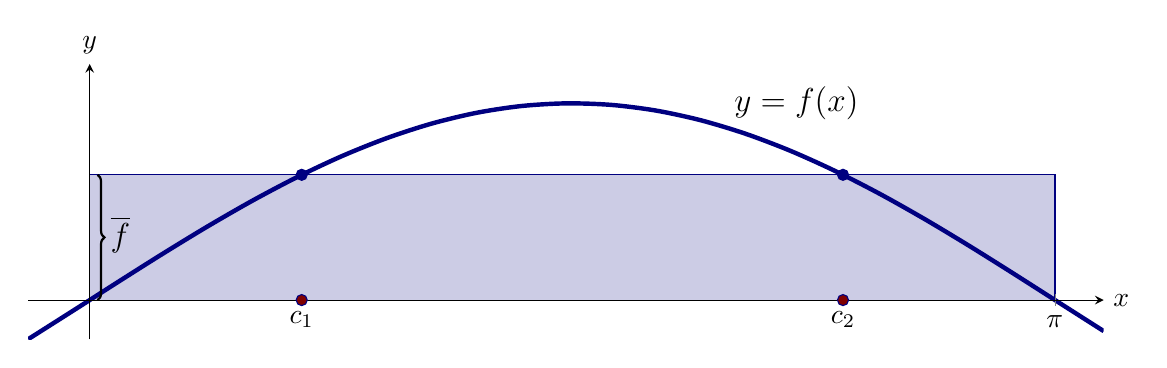
\begin{tikzpicture}[
      declare function = {f(\x) = sin(deg(\x));}]
    \begin{axis}[  
        domain=-.2:3.3, xmin =-.2,xmax=3.3,ymax=1.2,ymin=-.2,
        width=6in,
        height=2in,xtick={3.141,6.282},
        xticklabels={$\pi$, $2\pi$},
        ytick style={draw=none},
        yticklabels={},
        axis lines=center, xlabel=$x$, ylabel=$y$,
        every axis y label/.style={at=(current axis.above origin),anchor=south},
        every axis x label/.style={at=(current axis.right of origin),anchor=west},
        axis on top,
      ]
	\addplot [draw=penColor,fill=fillp] plot coordinates
                          {({0},{2/pi})
                            ({pi},{2/pi})} \closedcycle;
               \addplot [ultra thick,penColor, smooth] {f(x)};
 \addplot[color=penColor,fill=penColor2,only marks,mark=*] coordinates{(0.69,0)};  %% closed hole   
  \addplot[color=penColor,fill=penColor,only marks,mark=*] coordinates{(0.69,2/pi)};  %% closed hole  
   \addplot[color=penColor,fill=penColor,only marks,mark=*] coordinates{(pi-0.69,2/pi)};  %% closed hole    
      \addplot[color=penColor,fill=penColor2,only marks,mark=*] coordinates{(pi-0.69,0)};  %% closed hole   
       \addplot[decoration={brace,mirror,raise=.1cm},decorate,thick] plot coordinates
                       {(0,0) (0,2/pi)};
        \node[black] at (axis cs:0.69,-0.1) {$c_1$};
         \node[black] at (axis cs:pi-0.69,-0.1) {$c_2$};
           \node[black] at (axis cs:0.1,1/3) {\large$\overline{f}$};
             \node[black] at (axis cs:2.3,1) {\large$y=f(x)$};
    \end{axis}
  \end{tikzpicture}
\end{image}
  \end{explanation}
\end{example}
\end{document}
